\documentclass[12pt]{article}

% different fontsize than 10pt (default)
% article only supports 10, 11 and 12
% \documentclass[twocolumn, 9pt]{extarticle}

%%%%%%%%%%%%%%%%%%%%%%%%%%%%%%%%%%%%%%%%%%%%%%%%%%%%%%%%%%%%%%%%%%%%%%%%%%%%%%%%
%%%%%%%%%%%%%%%%%%%%%%%%%%%%%%%% PACKAGES %%%%%%%%%%%%%%%%%%%%%%%%%%%%%%%%%%%%%%
%%%%%%%%%%%%%%%%%%%%%%%%%%%%%%%%%%%%%%%%%%%%%%%%%%%%%%%%%%%%%%%%%%%%%%%%%%%%%%%%

% Font support, czech language
% czech babel... date, image descriptions etc. switch to czech
\usepackage[czech]{babel}
\usepackage[utf8]{inputenc}
\usepackage[T1]{fontenc}
\usepackage{fontspec}

\usepackage[a4paper, margin=2cm]{geometry}

% Math symbols (mathbb)
\usepackage{amsmath}
\usepackage{amssymb}
% \usepackage{amsfonts}

% Images (put into img/ subdirectory)
\usepackage{graphicx}
\graphicspath{{img/}}

% links (href)
\usepackage[pdfusetitle]{hyperref}

% Lorem ipsum by \lipsum[1-n] for n paragraphs
% \usepackage{lipsum}
\usepackage[text=lipsum-cs]{lipsum}

% http://www.ctan.org/pkg/algorithms
%\usepackage{algorithmic}

%\usepackage{array}

%%%%%%%%%%%%%%%%%%%%%%%%%%%%%%%%%%%%%%%%%%%%%%%%%%%%%%%%%%%%%%%%%%%%%%%%%%%%%%%%
%%%%%%%%%%%%%%%%%%%%%%%%%%%%%%%% DEFINITIONS %%%%%%%%%%%%%%%%%%%%%%%%%%%%%%%%%%%
%%%%%%%%%%%%%%%%%%%%%%%%%%%%%%%%%%%%%%%%%%%%%%%%%%%%%%%%%%%%%%%%%%%%%%%%%%%%%%%%

% paragraph style... first line indent, space between paragraphs
% \setlength{\parindent}{0pt}
% \setlength{\parskip}{10pt}

% \newcommand{\etal}{\emph{et al.} }

%%%%%%%%%%%%%%%%%%%%%%%%%%%%%%%%%%%%%%%%%%%%%%%%%%%%%%%%%%%%%%%%%%%%%%%%%%%%%%%%
%%%%%%%%%%%%%%%%%%%%%%%%%%%%%%%% DOCUMENT %%%%%%%%%%%%%%%%%%%%%%%%%%%%%%%%%%%%%%
%%%%%%%%%%%%%%%%%%%%%%%%%%%%%%%%%%%%%%%%%%%%%%%%%%%%%%%%%%%%%%%%%%%%%%%%%%%%%%%%

\title{SIMages -- Podobnostní spojení na databázi obrázků}

\author{
    Šimon Růžička, FIT ČVUT\\
    \texttt{ruzicsi1@fit.cvut.cz}
    }
% \date{}

\begin{document}
\maketitle

%%%%%%%%%%%%%%%%%%%%%%%%%%%%%%%%%%%%%%%%%%%%%%%%%%%%%%%%%%%%%%%%%%%%%%%%%%%%%%%%
\section*{Zadání}

Cílem projektu je vytvoření webové aplikace, která umožní podobnostní spojení dvou sad obrázků s využitím
rozsahového dotazu (range query) a dotazu na k nejbližších sousedů (k-nearest neighbor (kNN) query).

% \vspace{2em}
% \noindent
\section*{Prohlášení}

Projekt byl zadán jako semestrální práce v rámci předmětu BI-VWM.21%
\footnote{\url{https://bk.fit.cvut.cz/cz/predmety/00/00/00/00/00/00/06/70/24/p6702406.html}}.
Rád bych poděkoval Ing. Jiřímu Novákovi, Ph.D. (\texttt{jiri.novak@fit.cvut.cz}) za konzultace práce v rámci cvičení tohoto předmětu.

%%%%%%%%%%%%%%%%%%%%%%%%%%%%%%%%%%%%%%%%%%%%%%%%%%%%%%%%%%%%%%%%%%%%%%%%%%%%%%%%
\section{Úvod}

Semestrální práce implementuje webovou aplikaci pro podobnostní spojení jednoho obrázku, tzv. klíče, se sadou obrázků.
Aplikace nahraje dostupné sady obrázků z příslušného adresáře a umožní uživateli interaktivní výběr klíče a sady obrázků.
Zároveň má uživatel k dispozici několik parametrů vyhledávání, jako je výběr predikátu (kNN, rozsahový) a jeho parametru nebo výběr metriky (cosinová podobnost, Euklidovská vzdálenost).
Uživateli se následně na nové obrazovce zobrazí jeho zvolený klíčový obrázek, společně se spojenými obrázky seřazenými od nejpodobnějších podle zvolené metriky.

Po dokončení dotazu má uživatel možnost jej nadále upravovat, buď změnou parametrů vyhledávání nebo výběrem nového klíčového obrázku.
Pro přehlednost aplikace vždy zobrazuje pouze podobnostní spojení pro jeden klíčový obrázek.
Aplikace se tímto přístupem snaží simulovat vzhled doporučovacích algoritmů různých webových služeb.
Jedná se tedy o jednoduchý algoritmus doporučování na základě obsahu, který by pro praktické použití v on-line službě mohl být doplněn např. o algoritmus kolaborativního filtrování, tedy doporučení na základě aktivity jiných uživatelů.

Obrázky jsou porovnávány na základě deskriptorů vygenerovaných konvoluční neuronovou sítí VGG-16%
\footnote{\href{https://arxiv.org/abs/1409.1556}{Very Deep Convolutional Networks for Large-Scale Image Recognition, arXiv:1409.1556}}.
Použitá technika je detailněji popsána v sekci \ref{sec:generovani-deskriptoru}.

%%%%%%%%%%%%%%%%%%%%%%%%%%%%%%%%%%%%%%%%%%%%%%%%%%%%%%%%%%%%%%%%%%%%%%%%%%%%%%%%
\section{Způsob řešení}

Z algoritmického hlediska by se dal projekt rozdělit na dva odlišné procesy.
Jedná se o předzpracování dat v podobě generování deskriptorů pomocí neuronové sítě (sekce \ref{sec:generovani-deskriptoru}) a samotné vyhodnocení dotazu (sekce \ref{sec:vyhodnoceni-dotazu}).

Předzpracování dat neuronovou sítí je na běžném stroji pro větší sady obrázků časově náročné.
Tento proces však stačí provést pouze jednou, a to při nahrávání samotné sady obrázků, případně při jejím rozšíření o nové obrázky.
Po tomto výpočtu se všechny deskriptory uloží do komprimovaného souboru \texttt{features.npz}, odkud se následně načítají při provádění dotazu.
V ideálním případě tedy proces proběhne na pozadí, aniž by zdržoval uživatelskou aktivitu.

Pro vyhodnocení dotazu je potřeba porovnávat známý klíčový obrázek s každým obrázkem ve zvolené sadě za použití předpočítaných deskriptorů.
Algoritmus byl vyladěn tak, aby byl dostatečně responzivní pro použití za běhu aplikace.
Pro větší data je možné, že by bylo potřeba dotazovací algoritmus optimalizovat, možnosti jsou popsány v sekci \ref{sec:moznosti-optimalizace}.

Bližší podrobnosti o rychlosti těchto operací jsou popsány v sekci \ref{sec:experimentalni-sekce}.

\subsection{Generování deskriptorů}\label{sec:generovani-deskriptoru}

Algoritmus pro generování deskriptorů využívá konvoluční neuronovou síť VGG-16, respektive její předpřipravenou implementaci v balíčku Keras%
\footnote{\url{https://keras.io/api/applications/vgg/}}.
Tato síť byla původně navržena a natrénována pro klasifikaci obrázků z datové sady ImageNet v rámci soutěže ILSVRC%
\footnote{\url{https://image-net.org/challenges/LSVRC/}}.
Samotné fungování neuronové sítě přesahuje znalosti relevantní pro tento předmět a tuto semestrální práci.
Pokud však z neuronové sítě odejmeme poslední vrstvu, která generuje samotné pravděpodobnosti jednotlivých tříd datasetu ImageNet, dostaneme vektor hodnot (fakticky trojrozměrný tensor, výška $\times$ šířka $\times$ počet kanálů) reprezentující obrázek.
Technice použití natrénovaných neuronových sítí na zcela jiných datech nebo za jiným účelem se přezdívá \emph{transfer learning}.

Nad tímto vektorem předposlední vrstvy neuronové sítě tedy můžeme uvažovat stejně, jako nad deskriptory konvenční metody zpracování obrazu.
V případě sítě VGG-16 má výstup rozměry $7 \times 7 \times 512$, tedy celkem 25088 32-bitových desetinných čísel.
V důsledku fungování sítě je však tento vektor řídký, v průměru je přibližně z 90 \% tvořen nulami.
Toho bychom mohli využít vhodnou reprezentací, která by ušetřila výpočetní čas i velikost ukládaných souborů, tato možnost je diskutována v sekci \ref{sec:moznosti-optimalizace}.

Pro ukládání deskriptorů byla použita knihovní funkce \texttt{numpy.savez\_compressed}%
\footnote{\url{https://numpy.org/doc/stable/reference/generated/numpy.savez_compressed.html}},
která využívá kompresního algoritmu \texttt{gzip}.
Tento algoritmus již dokáže využít řídkosti deskriptorů, experimentálně se ukázalo že zmenšil velikost souboru s deskriptory zhruba osminásobně.

\subsection{Vyhodnocení dotazu}\label{sec:vyhodnoceni-dotazu}

Při vyhodnocení dotazu je nejprve potřeba porovnat vektor deskriptorů klíčového obrázku s jednotlivými vektory ve zvolené datové sadě.
K tomu se používá jedna ze zvolených metrik, cosinová podobnost nebo Euklidovská vzdálenost.
Metriky se liší především v pořadí záznamů -- dotaz má prioritně vracet obrázky s maximální podobností, nebo s minimální vzdáleností.
Dalším rozdílem je také citlivost Euklidovské vzdálenosti vůči škálování, zatímco cosinová podobnost uvažuje všechny $k$-násobky vektoru jako identické a vnímá pouze jeho směr.

Zvolený přístup k samotnému vyhodnocení je pak poměrně naivní -- uvažujeme dvojice klíčového obrázku s každým obrázkem v sadě, vypočítáme sledovanou metriku a záznamy podle této metriky seřadíme.
Možné optimalizace jsou diskutovány v sekci \ref{sec:moznosti-optimalizace}.

Po korektním seřazení obrázků ještě přichází druhá fáze vyhodnocení, tou je aplikace samotného predikátu.
V případě kNN predikátu pouze ořízneme seřazené pole obrázků na požadovanou velikost, zadanou uživatelem.
V případě rozsahového predikátu nejprve spočítáme, kolik záznamů přesáhlo uživatelem nastavenou hranici, k tomu lze na seřazeném poli použít binární vyhledávání.
Tento nalezený počet následně nastavíme jako $k$ a pokračujeme stejně, jako u kNN predikátu.

\subsection{Možnosti optimalizace}\label{sec:moznosti-optimalizace}

Uvádíme některé z možných návrhů, které by mohly zrychlit běh programu (fázi vyhodnoceni dotazu), ale jejich implementace byla mimo časové možnosti této semestrální práce.

Řídká reprezentace deskriptorů by patrně nijak výrazně nezměnila jejich velikost na disku, díky použitému kompresnímu algoritmu.
Jejich použití by však potenciálně mohlo zrychlit fázi výpočtu metriky.
Jelikož pro výpočet metrik byly použity funkce z knihovny numpy, pak by pro řídkou reprezentaci bylo nejvhodnější použít kompatibilní typ \texttt{scipy.sparse}%
\footnote{\url{https://docs.scipy.org/doc/scipy/reference/sparse.html}}.

Pro optimalizované vyhodnocení dotazu by také bylo možné využít vlastností metrického prostoru.
Techniky využívající tabulek pivotů a hierarchie mezi jednotlivými záznamy jsou v principu nepochybně efektivnější, než naivní porovnání s každým dostupným záznamem.
Tento rozdíl by byl obzvláště znatelný pro větší počet fotek v jednom spojovaném adresáři.
Tyto techniky jsou detailněji popsány v 9. přednášce BI-VWM.21%
\footnote{\url{https://moodle-vyuka.cvut.cz/pluginfile.php/780673/course/section/111400/BIVWM_lecture09.pdf}}.

%%%%%%%%%%%%%%%%%%%%%%%%%%%%%%%%%%%%%%%%%%%%%%%%%%%%%%%%%%%%%%%%%%%%%%%%%%%%%%%%
\section{Implementace}

% Popsat jaké byly použity programovací jazyky, jaká je architektura aplikace, jaké
% knihovny byly použity, jaké jsou požadavky na spuštění aplikace, apod.

Celá implementace vznikla v programovacím jazyce Python ve verzi 3.12.
Pro generování obrázkových deskriptorů byl použit obecný framework pro strojové učení Keras s PyTorch backendem.
Následné vektorové operace, proces archivace vektorů a jejich porovnávání je implementováno převážně pomocí knihovny numpy.
Webové rozhraní pak zajišťuje knihovna NiceGUI.

Kompletní seznam použitých balíčků, včetně závislostí a všech verzí je obsažen v souboru \texttt{environment.yml}.
Tento soubor byl vygenerován manažerem vývojových prostředí Conda.
Kopii prostředí nutnou pro spuštění serveru aplikace lze vytvořit pomocí následujícího příkazu:

\begin{verbatim}
conda env create --file /path/to/environment.yml
\end{verbatim}

Pro spuštění klienta aplikace pak postačuje webový prohlížeč a síťové spojení se serverem, který provádí všechny výpočty.

\subsection{Architektura aplikace}

Aplikace je logicky rozdělená do několika modulů.
O výpočetní část práce se starají moduly \texttt{compute\_features.py} (generování deskriptorů) a \texttt{nearest.py} (vyhodnocení dotazu).
Generování dvou webových stránek pak obstarávají moduly \texttt{key\_select.py} a \texttt{similar\_results.py}, obsažené uvnitř adresáře \texttt{gui/}.
Program se spouští pomocí skriptu \texttt{\_\_main\_\_.py}, který je z důvodů multiprocessingu potřeba spustit napřímo, případně pomocí symbolického odkazu.

%%%%%%%%%%%%%%%%%%%%%%%%%%%%%%%%%%%%%%%%%%%%%%%%%%%%%%%%%%%%%%%%%%%%%%%%%%%%%%%%
\section{Příklady vstupu a výstupu}

% Screenshoty s popisem konkrétního vstupu a výstupu aplikace.
Webové rozhraní obsahuje celkem dvě webové stránky.
První slouží k prvotnímu nastavení vyhledávání a klíčového obrázku.
Druhá stránka pak v první řadě zobrazuje výsledek vyhledávání, lze na ní ale dotaz dodatečně upravit.

\subsection{Výběr klíčového obrázku}

\begin{figure}[h]
    \centering
    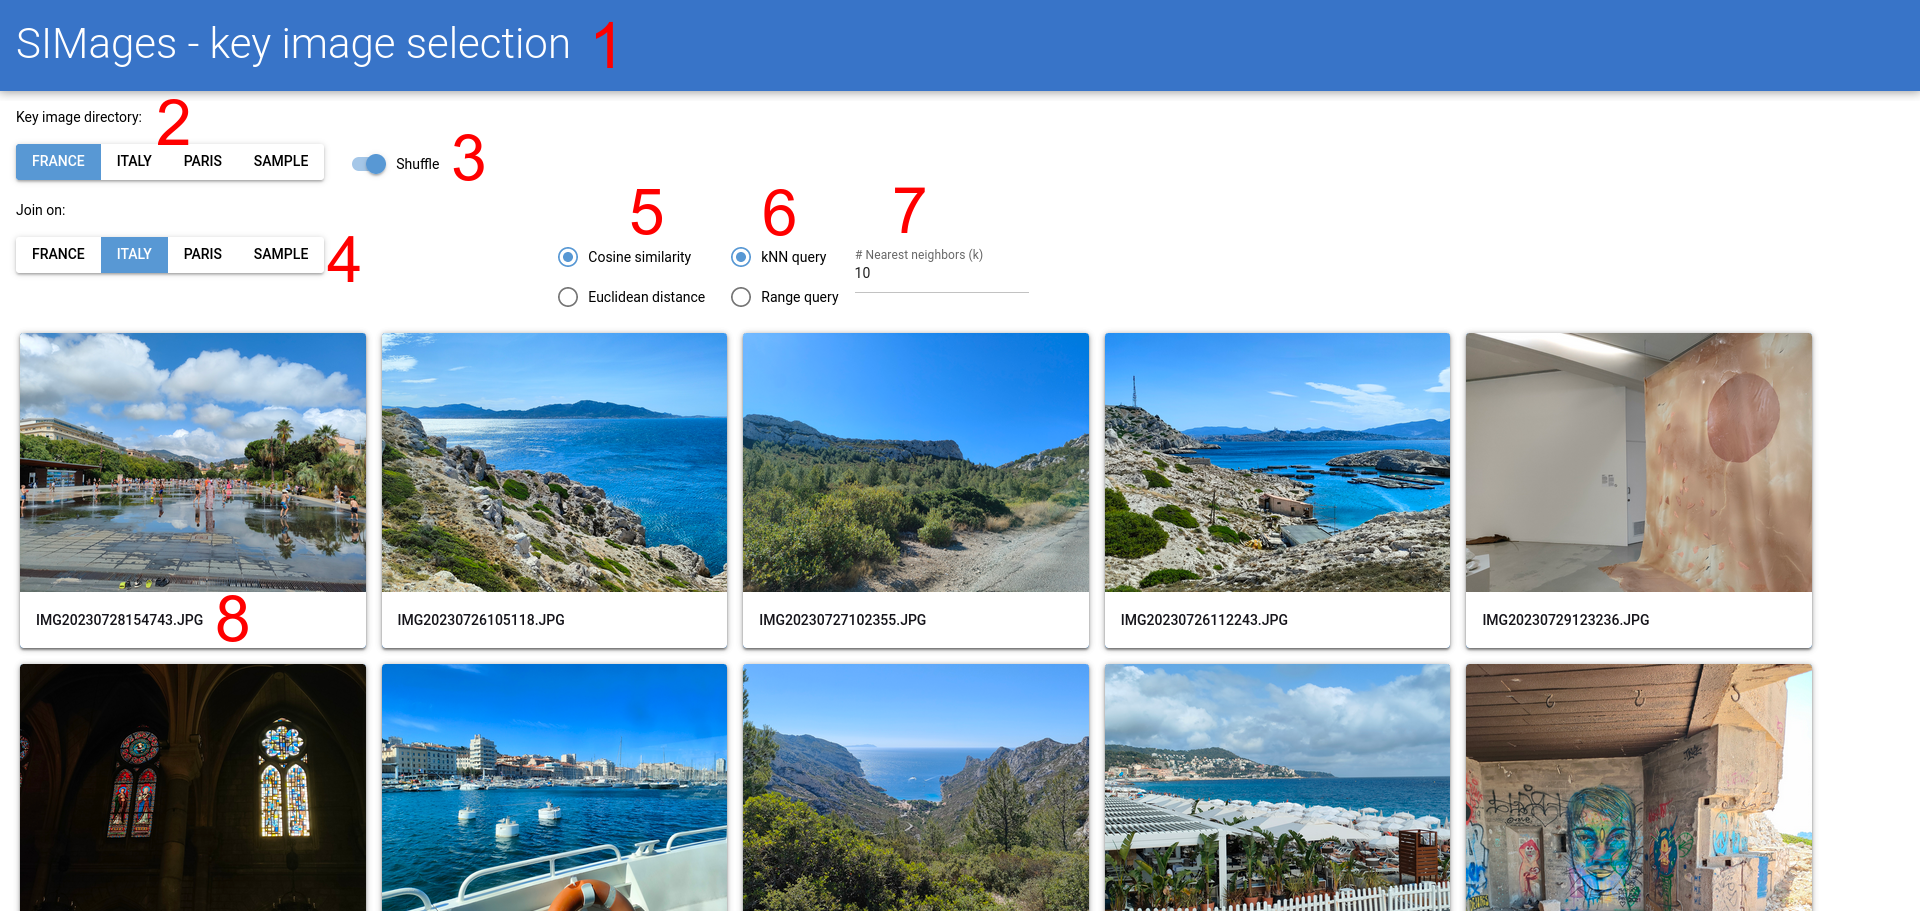
\includegraphics[width=0.9\linewidth]{key_selection_annotated.png}
    \caption{Úvodní stránka -- výběr klíčového obrázku}
    \label{fig:key-selection}
\end{figure}

Jednotlivé prvky stránky \ref{fig:key-selection}, jako označené v obrázku:

\begin{enumerate}
    \item Název stránky.
    \item Volba datové sady klíčového obrázku. Z této sady se načítá prezentovaný výběr obrázků, ihned po provedení volby.
    \item Možnost randomizovat pořadí obrázků ve výběru.
    \item Volba datové sady pro podobnostní spojení. Obrázky z této sady se budou zobrazovat na další stránce jako výsledky dotazu.
    \item Volba metriky podobnosti -- cosinová podobnost, Euklidovská vzdálenost.
    \item Volba predikátu -- kNN, rozsahový.
    \item Volba parametru predikátu, v závislosti na zvoleném predikátu a metrice.
    \item Výběr klíčového obrázku, zobrazuje se náhled a jméno souboru.
\end{enumerate}

\subsection{Výsledek dotazu}

\begin{figure}[h]
    \centering
    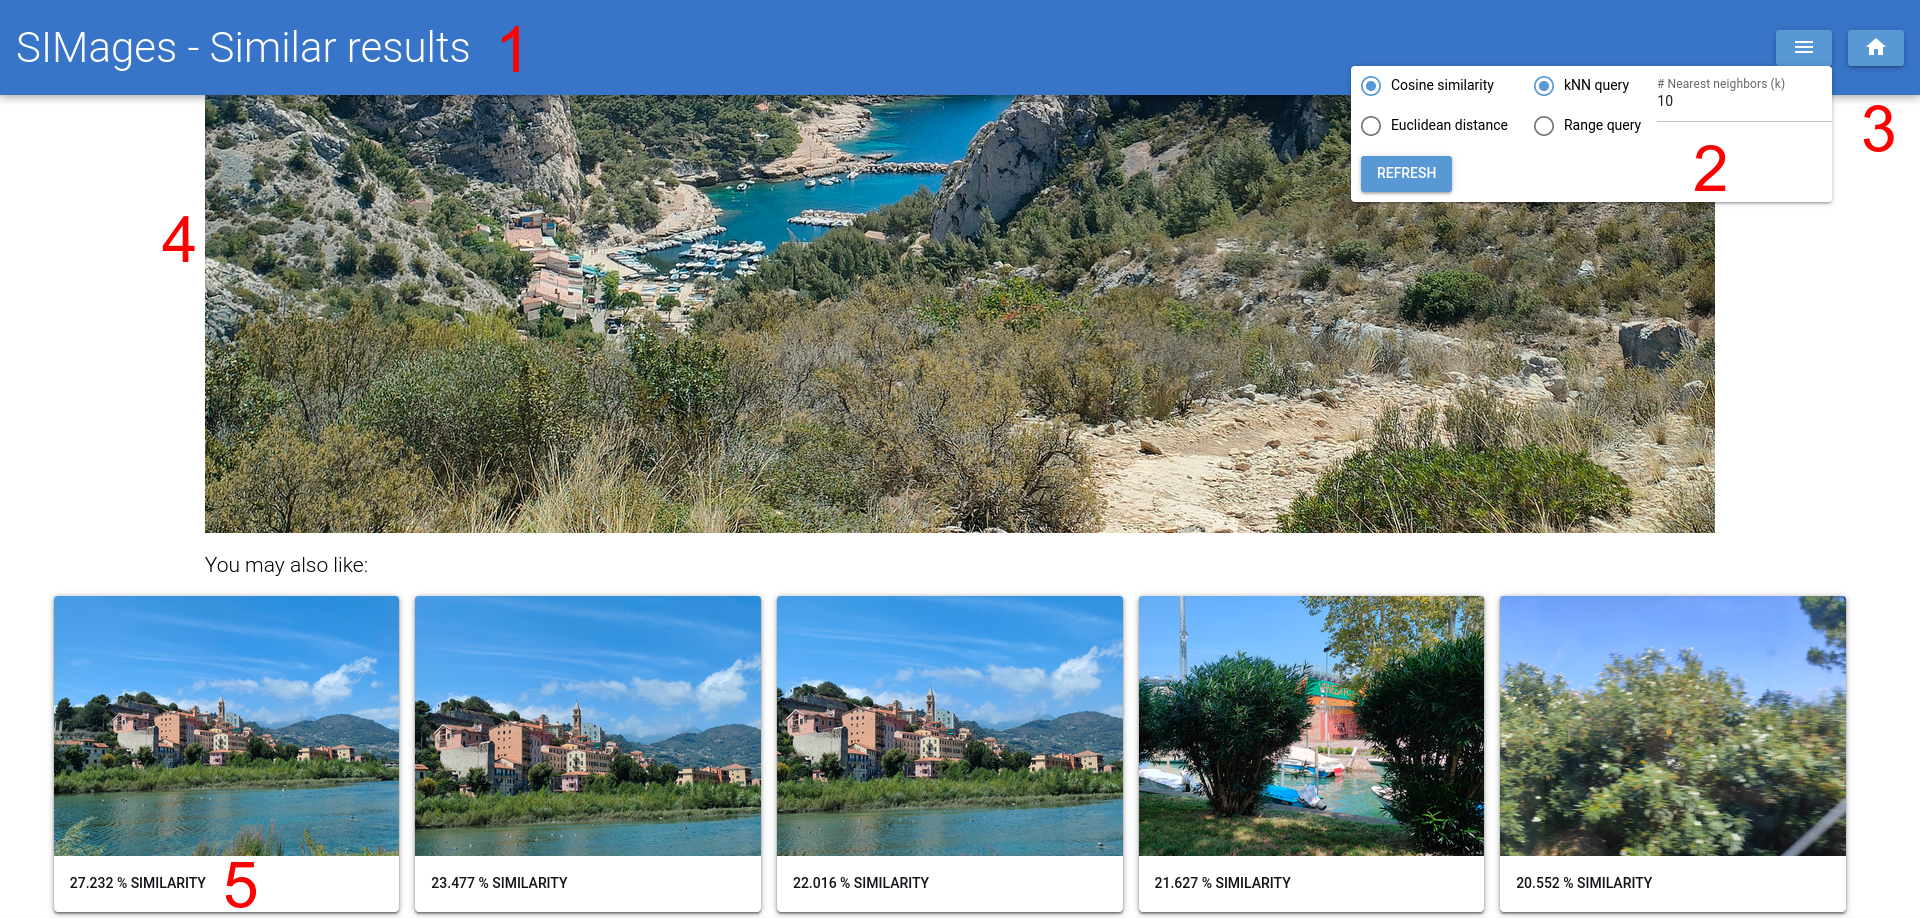
\includegraphics[width=0.9\linewidth]{similar_results_annotated.png}
    \caption{Stránka s výsledkem dotazu}
    \label{fig:similar-results}
\end{figure}

Jednotlivé prvky stránky \ref{fig:similar-results}, jako označené v obrázku:

\begin{enumerate}
    \item Název stránky.
    \item Rozbalovací nabídka s nastavením, shodné rozhraní jako na stránce \ref{fig:key-selection}, s přidaným potvrzovacím tlačítkem.
    \item Tlačítko pro návrat na předchozí domovskou stránku.
    \item Klíčový obrázek zvolený v předchozím kroku.
    \item Výsledek dotazu, seřazený podle relevantní metriky. Zobrazuje se náhled a výsledek metriky. Po prokliknutí se obrázek vykreslí přes celou obrazovku.
\end{enumerate}

%%%%%%%%%%%%%%%%%%%%%%%%%%%%%%%%%%%%%%%%%%%%%%%%%%%%%%%%%%%%%%%%%%%%%%%%%%%%%%%%
\section{Experimentální sekce}\label{sec:experimentalni-sekce}

% Většinu aplikací lze posuzovat z hlediska přesnosti a/nebo rychlosti. Obojí je závislé
% na různých vstupních parametrech projektu. V experimentech by měly být tyto
% parametry zkoumány. Např. rychlost typicky závisí na velikosti vstupního datasetu.
% Lze tedy vyrobit tabulku nebo graf se závislostí času na velikosti vstupního datasetu.

Provedli jsme časové testy na jednotlivé výpočetní operace, které aplikace provádí.
Všechny testy byly prováděny na běžném notebooku (procesor AMD Ryzen 4500U%
\footnote{\url{https://www.amd.com/en/product/9101}}),
bez použití GPU pro vyhodnocení neuronové sítě.

Testy ukázaly, že proces generování obrázkových deskriptorů trvá včetně režie načítání souborů přibližně 150 ms na obrázek.
Pro menší sady obrázků by byl čas ještě o něco vyšší, neuronové sítě jsou optimalizované na dávkové vyhodnocení, v tomto případě jsme zvolili velikost dávky 64.
Je tedy zjevné, že tento proces není realisticky proveditelný za běhu aplikace.
V tomto případě se také nenabízí žádné zjevné optimalizace v kódu, pouze použití většího výpočetního výkonu nebo kompletně jiného algoritmu.

Pro datové sady testované velikosti v rozmezí 200 až 300 obrázků trval jeden dotaz zhruba 250 ms v závislosti na parametrech.
To znamená, že byl dostatečně rychlý na použití za běhu aplikace.
S rostoucím počtem obrázků ve spojované datové sadě by doba vyhodnocení zjevně rostla asymptoticky lineárně; nejnáročnější operací je porovnávání deskriptorů klíčového obrázku s každým obrázkem ve spojované sadě.

Jelikož je vyhodnocení výsledku silně subjektivní, nebylo možné provést objektivní testy kvality výsledků.
Jednou z možností by bylo vytvořit testovací skupinu uživatelů, kterým by byly předloženy výsledky dotazu v porovnání s jinými prototypy, případně s konkurenčními službami.
Následně by se na základě průměrného hodnocení uživatelů dalo odvodit, který z algoritmů funguje "lépe".
Takový test není v možnostech této práce.

%%%%%%%%%%%%%%%%%%%%%%%%%%%%%%%%%%%%%%%%%%%%%%%%%%%%%%%%%%%%%%%%%%%%%%%%%%%%%%%%
\section{Diskuze}

% Většina projektů je typu “proof of koncept“, tj. jde o vyzkoušení poznatků
% prezentovaných v přednáškách v praxi. Nejde tedy o detailní řešení všech problémů,
% které mohou při implementaci nastat -- takový projekt by dalece přesahoval rámec
% semestrálního projektu. Tato sekce tedy obsahuje rozbor těchto nedostatků a
% možnosti jejich řešení.

Hlavní myšlenkou projektu bylo implementovat návrh algoritmu, který je schopný vyhledávat podobné obrázky na středně velké datové sadě, obsahující řádově stovky obrázků.
Tento algoritmus je stále možné optimalizovat, jak konceptuálně (vizte sekci \ref{sec:moznosti-optimalizace}) tak i efektivnější implementací.
Ačkoliv byly při implementaci prioritně používány funkce z relativně efektivních knihoven (numpy, scipy), Python se v žebříčcích rychlosti běhu programovacích jazyků obvykle umisťuje na zadních příčkách%
\footnote{\url{https://benchmarksgame-team.pages.debian.net/benchmarksgame/index.html}}.
Vhodným řešením by tedy bylo vytvořit implementaci v rychlejším kompilovaném jazyce (např. C/C++, Rust), která by byla následně volána z webserveru.
Podobné, optimalizace by bylo možné najít také na straně frameworku pro neuronové sítě PyTorch, jako například přechod z JIT na kompilovaný model%
\footnote{\url{https://pytorch.org/tutorials/intermediate/torch_compile_tutorial.html}}.

Bylo by také možné zlepšit kvalitu výsledků pomocí dříve uvedených testů s lidskou evaluací modelu (sekce \ref{sec:experimentalni-sekce}).
Pravděpodobně by bylo vhodné experimentovat s komplexnějšími metodami zpracování obrázku, jako jsou různé transformace před vstupem doo neuronové sítě.
Příkladem může být postup autorů VGG-16, který z obrázku vyberou několik automatických výřezů, které jednotlivě vstupují do neuronové sítě, výsledná predikce je pak tvořena průměrem těchto dílčích predikcí.

%%%%%%%%%%%%%%%%%%%%%%%%%%%%%%%%%%%%%%%%%%%%%%%%%%%%%%%%%%%%%%%%%%%%%%%%%%%%%%%%
\section{Závěr}

% Stručné shrnutí toho, co se řešilo, zhodnocení výstupů projektu.

Samotný princip podobnostního spojování obrázků je využitelný v mnoha různých aplikacích.
Nejčastější využití však obnáší spojení velké sady se sebou samotnou (tzv. self-join), např. všechen obsah na sociální síti nebo obrázky indexované vyhledávačem.
Uživateli je možné po zobrazení obrázku (feed sociální sítě, vyhledávání) nabídnout podobný obsah, který pro něj může být užitečný, udrží jeho pozornost na síti, atd.
Podobné techniky pravděpodobně webové vyhledávače využívají pro tzv. query-by-example, kde je fulltextový dotaz ve vyhledávání nahrazen obrázkem.

Navržený prototyp je funkční pro menší datové sady (řádově stovky obrázků), jeho největším kamenem úrazu pro praktické využití je optimalizace.
Obsahuje webové rozhraní, ve kterém je možné zvolit klíčový obrázek, spojovanou sadu a jiné parametry vyhledávání (typ metriky, typ dotazu/"predikát").

%%%%%%%%%%%%%%%%%%%%%%%%%%%%%%%%%%%%%%%%%%%%%%%%%%%%%%%%%%%%%%%%%%%%%%%%%%%%%%%%
%%%%%%%%%%%%%%%%%%%%%%%%%%%%%%%% TEMPLATES %%%%%%%%%%%%%%%%%%%%%%%%%%%%%%%%%%%%%
%%%%%%%%%%%%%%%%%%%%%%%%%%%%%%%%%%%%%%%%%%%%%%%%%%%%%%%%%%%%%%%%%%%%%%%%%%%%%%%%

% https://tex.stackexchange.com/questions/89462/page-wide-table-in-two-column-mode
% \begin{table*}[t]
%     \centering
%     \begin{tabular}{|llll|l|}
%         \hline
%         Square meters & Distance from center & Distance from U-Bahn & Garden & Price \\
%         \hline
%         $x_1$ & $x_2$ & $x_3$ & $x_4$ & $y$ \\
%         \hline
%         105 m$^2$     & 2.3 km      & 0.3 km & 0     & 582 463 €     \\
%         \hline
%     \end{tabular}
% \end{table*}

% \lipsum[3-5]

% \begin{itemize}
%     \item země je v Eurozóně -- kategorický regresor
%     \item země byla v minulosti součástí tzv. Východního bloku \footnote{
%         Za státy Východního bloku budeme považovat ty, které byly v minulosti
%         členem Varšavské smlouvy. Případné změny státních hranic budou dále níže
%         diskutovány.}
%      -- kategorický regresor
%     \item počet obyvatel -- spojitý regresor, Eurostat kód \texttt{demo\_r\_pjanaggr3}
%         \footnote{\href{https://ec.europa.eu/eurostat/cache/metadata/en/demo_r_gind3_esms.htm}
%         {Odkaz na dataset \texttt{demo\_r\_pjanaggr3}.}}.
%     \item průměrná hrubá mzda -- spojitý regresor, Eurostat kód \texttt{earn\_nt\_net}
%         \footnote{\href{https://ec.europa.eu/eurostat/cache/metadata/en/earn_net_esms.htm}
%         {Odkaz na dataset \texttt{earn\_nt\_net}.}}.
% \end{itemize}

% \lipsum[6]

% \begin{equation}
%     \begin{aligned}
%         \mathcal{L}^{(i)} &= \text{ReLU}(\mathcal{L}^{(i-1)}) = \max(0,\mathcal{L}^{(i-1)})\\
%         R^{(i-1)}_{\text{backprop}} &= (\mathcal{L}^{(i-1)} > 0) \cdot R^{(i)}\\
%         R^{(i-1)}_{\text{guided}} &= (R^{(i)} > 0) \cdot (\mathcal{L}^{(i-1)} > 0) \cdot R^{(i)}
%     \end{aligned}
% \end{equation}

% \lipsum[7]

% \begin{figure}[h]
%     \centering
%     \includegraphics[width=0.9\linewidth]{image_file_name}
%     \caption{Image caption}
%     \label{fig:image_label}
% \end{figure}

\end{document}